\section{Introduction}

The purpose of this assignment is to improve a sequential version of an image processing algorithm on a multi-core heterogeneous computing platform provided. The given platform is the Beagle Board\footnote{http://beagleboard.org/} that has a general purpose ARM processor (from now on referred to as the \emph{GPP}) and a digital signal processor (\emph{DSP}) that would be utilized in this lab for the edge detection algorithm and eventually obtaining a speed up by performing computations in parallel. Luckily the heavily used gaussian filtering function (see \hyperref[sec:profiling]{section~\ref{sec:profiling}). Profiling}) could be load balanced among different processing units due to its very little data dependency. In the following sections we will describe the difficulties of working with this system, go into some depth about the obtained speedup and discuss further improvements that could be made.

\subsection{Overview}
Figure~\ref{fig:workflow} shows the reader the overall approach to this problem and the basic work flow that we adhered to. In this report we will go through describing each component in the flow diagram presented. We would also discuss the communication model that was used to communicate the necessary data in the heterogeneous environment, and see that the communication model (i.e. shared memory) used here has little overhead and imposes almost no additional delays when compared to the communication model (i.e. message passing) that was utilized in the previous lab.

The application profiling has made a great impact on steering our decisions as we will see in \hyperref[sec:profiling]{Section~\ref{sec:profiling}}. Furthermore every core has a hardware limitation in terms of how many operations can be performed at the same time, which defines the upper bound on how much speed-up can be obtained. The results along with the corresponding error analysis are presented. Lastly, further improvements that could potentially improve the execution speed of the application are discussed in the future improvements section.

\begin{figure*}
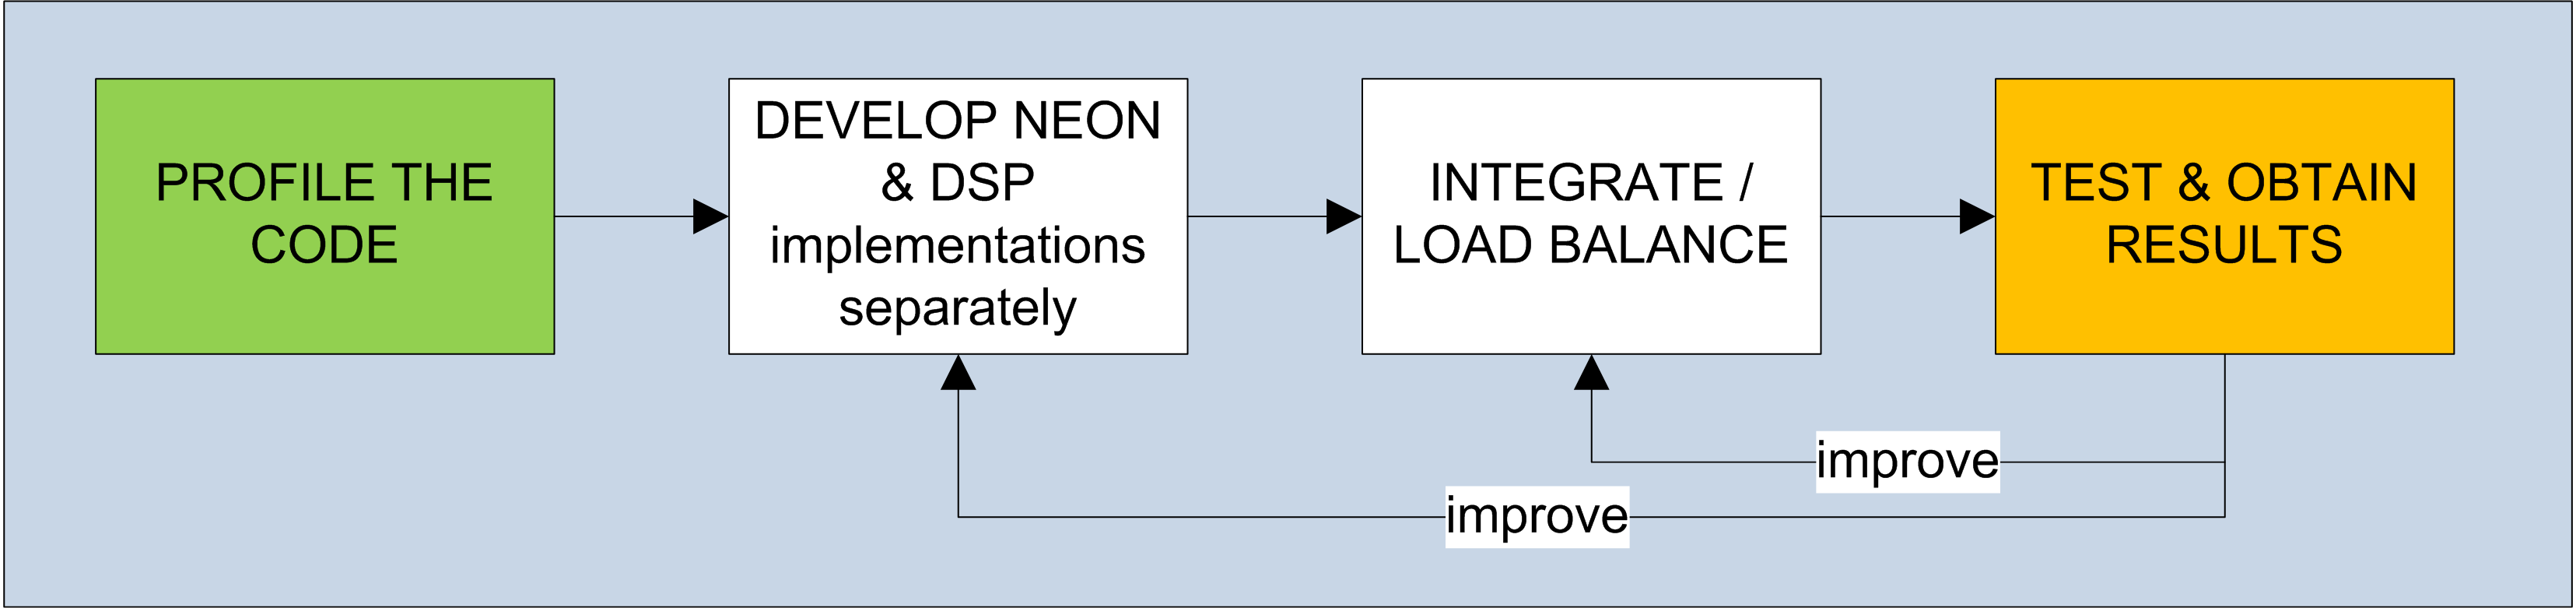
\includegraphics[width=\linewidth]{drawings/workflow}
\caption{General approach to the problem}
\label{fig:workflow}
\end{figure*}


